\chapter{Mechanik}

\renewcommand{\kapitelautor}{Autor: Alexander Punz}

\section{Allgemeine technische Planung}

		\subsubsection{Allgemeine Informationen über 3D Drucken}

		Die Technologie des 3D Druckens hat in den letzten Jahren immer mehr an Popularität gewonnen. Mit Hilfe des 3D Druckers kann man fast alle vorstellbaren Formen anfertigen.
		Es gibt verschiedenste Verfahren wie man ein Werkstück anfertigen kann: Laser Sintern, Stereolithographie, Drucken mit flüssigen Materialien, etc.
		In diesem Projekt wird nur die Variante des Druckens mit flüssigen Material verwendet.
		Diese ist kostengünstig \bzw. genau genug für die Teile. Wie der Name schon sagt, wird Material in einem Druckkopf geschmolzen und dann Schicht für Schicht auf der Druckplatte aufgetragen.
		Der Druckkopf fährt nur in X und Y Richtung, die Höhe wird mit der Druckplatte selbst verfahren.

		Meist werden Drucker über einen Maschinencode gesteuert, dem sogenannten „G-Code“. In diesem Code werden die Punkte (Koordinaten) definiert, die der Extruder (Druckkopf) abfahren muss.
		Die folgende Abbildung zeigt ein Beispiel eines Maschinencodes.

			\begin{figure}[tbh]
			\begin{centering}
			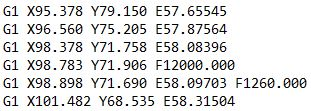
\includegraphics[width = 0.4\textwidth]{Bilder/gcode_erklaerung}
			\par\end{centering}
			\caption{Maschinencode Erklärung}
			\label{gcode}
			\end{figure}

			% Table generated by Excel2LaTeX from sheet 'Tabelle1'
			\begin{table}[htbp]
  		\centering
  		\caption{Befehle G Code}
	    \begin{tabular}{ll}
	    G1    & Kontrollierte Bewegung \\
	    X, Y  & Koordinaten in horizontaler und vertikaler Richtung \\
	    E     & Angabe der Menge des Filaments, dass in den Extruder geschoben werden muss \\
	    F     & Geschwindigkeit, mit der das Material in den Extruder geschoben wird (mm/min) \\
	    \end{tabular}%
	  	\label{tab:befehle gcode}%
			\end{table}%

		\subsubsection{Materialeigenschaften}

		\subsubsection{Von der Idee zur Anfertigung}

\section{Halterung für Cupcakes}

	\subsection{Technische Planung}

	\subsection{Umsetzung}

	\subsection{Herausforderungen und Lösungen}

	%\subsection{Implementierung}

\section{Rotorschutz}

	\subsection{Technische Planung}

	\subsection{Umsetzung}

	\subsection{Herausforderungen und Lösungen}

	\subsection{Implementierung}

\section{Halterung Ultraschallsensor}

	\subsection{Technische Planung}

	\subsection{Umsetzung}

	\subsection{Implementierung}

\section{Halterung PIXY cmucam5}

	\subsection{Technische Planung}

		\subsubsection{Berechnungen}

	\subsection{Umsetzung}

	\subsection{Implementierung}

	\subsection{Testphase}

\section{Führung für Testflüge}

	\subsection{Technische Planung}

	\subsection{Umsetzung}

	\subsection{Implementierung}

	\subsection{Testphase}

\section{Persönliche Erfahrungen}
